Ein Wegplanungs-Algorithmus kann entweder verteilt oder zentral arbeiten. Ein zentraler Algorithmus hat aber das Problem, dass der Berechnungsaufwand quadratisch von der Anzahl der Agenten abhängig ist (TODO Quelle). Ist für diese Arbeit also nicht interessant, da ein potentiell stark skalierendes Agenten-System zum Einsatz kommt. Ein echtzeitfähiger, verteilter und skalierender Algorithmus ist der \textit{CoDy Algorithmus}. Der CoDy Algorithmus berechnet die Wege für jeden Agenten aus Sicht der jeweiligen Agenten und löst mit Hilfe von heuristischer Prioritätsanpassung auftretende Konflikte. Der \textit{CoDy Algorithmus} hat bestimmte Voraussetzungen an das implementierende System. Es soll verteilt sein, muss den Agenten die Möglichkeit bieten, untereinander zu kommunizieren und homogen sein. Zusätzlich muss ein Agent in der Lage sein seine Umgebung zu erfassen, entweder durch die eigene Sensorik oder durch Kommunikation mit anderen Agenten. Alle Voraussetzungen können erfüllt werden. \cite{book:regele}

Die Funktionsweise des CoDy Algorithmus wird in den folgenden Unterkapiteln genauer beschrieben. Es soll aber nicht Sinn dieser Arbeit sein, die Dissertation wiederzugeben. Die grundlegenden Elemente und Funktionen werden nicht nur zum Grundverständnis wiedergegeben. Vor allem soll aber eine Basis geschaffen werden, auf deren Grund dann im Kapitel (TODO link) beschrieben werden kann, wie der Algorithmus umgesetzt wird und wo es zu Abweichungen kommt.
\subsection{Grundlagen}
\label{chap:grundlagen}
In diesem Kapitel werden die grundlegenden Mechanismen und Elemente des CoDy Algorithmus vorgestellt.

\subsubsection{Das Weltmodell}
\label{chap:weltmodell}
Das Weltmodell ist zeitlich und räumlich diskret. Der CoDy Algorithmus kann mit jedem Weltmodell arbeiten, das sich als ungerichteter Graph darstellen lässt. Um die Berechnungen und Anschauungen aber nicht unnötig komplex zu gestalten, beschränkt sich das Weltmodell auf ein klassisches zweidimensionales Gitter. Die Zellen des Gitters sind quadratisch. Die Nachbarschaftsbeziehungen der Zellen beschränken sich auf vier Himmelsrichtungen. Sprich Zellen, die diagonal zu einander liegen, gelten nicht als benachbart. Eine Zelle kann verschiedene Zustände einnehmen. Die Zustände variieren jedoch zwischen Kartentypen. Sie werden deshalb in den folgenden Kapiteln erörtert. Ein weiteres Attribut der Zellen ist, dass sie eine bestimmte räumliche Größe haben. Für diese Arbeit wird jedoch angenommen, dass die Zellen ein wenig größer als die Agenten sind. Dies ist das einfachst anzunehmende Modell. \cite{book:regele}
%
\subsubsection{Die Entfernungskarte}
\label{chap:entfernungskarte}
Jeder Agent hält eine individuelle Entfernungskarte. Die grundlegende Aufgabe dieser Karte ist es, die Entfernung zum Ziel des Agenten wiederzugeben. Sie ist als Tabelle zu verstehen, in der für jede Zelle notiert ist, wie viele Bewegungsschritte nötig wären, um das Ziel von dieser Zelle aus zu erreichen. Diese Entfernungen werden durch eine einfache Breitensuche ermittelt. Die aktuelle Position des Agenten ist dabei nicht interessant. Der CoDy Algorithmus ist auch in der Lage mit unbekannten Umgebungen umzugehen. \cite{book:regele} \newline Zum einen ist das für den Anwendungsfall in erster Linie nicht interessant und zum anderen würde dies die Komplexität unnötig erweitern. Deshalb ist eine Entfernungskarte, im Kontext dieser Arbeit, eine Karte, die die gesamte Umgebung erfasst.
\begin{figure}[H]
    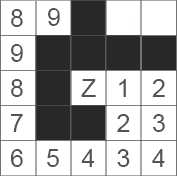
\includegraphics[height=40mm]{images/example_distancemap.png}
    \centering
    \caption{Beispiel für eine kleine Entfernungskarte}
    \label{fig:example_distancemap}
\end{figure}
Abbildung \ref{fig:example_distancemap} zeigt beispielhaft eine Entfernungskarte. Die grauen Zellen stellen statische Hindernisse dar. Das "'Z"' ist das Ziel des Agenten. Die Zahlen sind die Entfernungen und weiße Zellen sind nicht erreichbar.
%
\subsubsection{Die Umgebungskarte}
\label{chap:umgebungskarte}
\begin{figure}[H]
    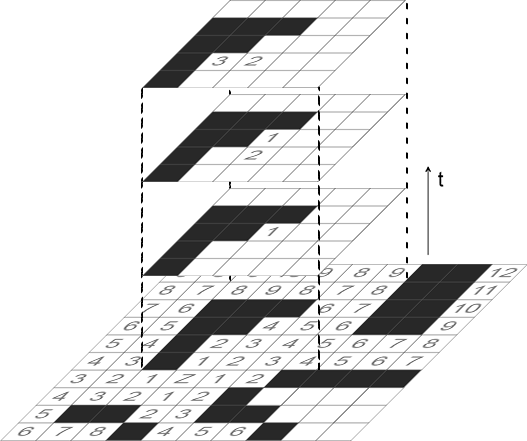
\includegraphics[width=9cm]{images/distance_localmap.png}
    \centering
    \caption{Entfernungs- und Umgebungskarte}
    \label{fig:distance_localmap}
\end{figure}
Die Umgebungskarte bildet einen Ausschnitt aus der Entfernungskarte dar. Im Gegensatz zur Entfernungskarte besitzt die Umgebungskarte eine Zeitdimension (siehe Abbildung \ref{fig:distance_localmap}). Damit ist es möglich dynamische Objekte, also andere Agenten, in die Wegplanung mit einzubeziehen. Dies beschreibt auch die Hauptfunktion dieser Karte. In die Umgebungskarte werden die, über Nachrichten von den anderen Agenten übermittelten, geplanten Wege eingetragen und für die eigene Wegplanung bereitgestellt. Die Dimensionen der Umgebungskarte sind immer ungerade, da die mittlere Zelle die aktuelle Position des Agenten spiegelt. Die Zeitdimension \(t\) zeigt von dem aktuellen Zeitpunkt aus in die Zukunft, wird aber durch die zeitlichen Berechnungstiefe \(t\textsubscript{max}\) begrenzt. Abbildung \ref{fig:distance_localmap} zeigt, dass die statischen Hindernisse von der Entfernungskarte übernommen werden, die Entfernungen jedoch nicht. Die Zellen halten andere Daten. Eine Zelle der Umgebungskarte ist entweder frei, von einen statischen Hindernis belegt oder von einem anderen Agenten reserviert. \cite{book:regele}
%
\subsubsection{Die Erreichbarkeitskarte}
\label{chap:erreichbarkeitskarte}
Die Erreichbarkeitskarte ist eine Erweiterung der Umgebungskarte und wird bei der Planung des eigenen Wegs erstellt. Sie gibt für jeden Zeitpunkt Auskunft, welche Zellen mit wie vielen Wegschritten von der aktuellen Position aus erreichbar sind. Da nicht davon auszugehen ist, dass ein Agent eine Zelle in einem Zeitschritt vollständig verlässt und die benachbarte Zelle vollständig betritt, muss der planende Agent seine Bewegungsschritte für \(t\) und \(t + 1\) reservieren. Das hat zur Folge, dass Agenten nicht direkt hintereinander fahren können und ist einer der beiden Mechanismen, wie Kollisionen zwischen den Agenten verhindert werden. \cite{book:regele}
\begin{figure}[H]
    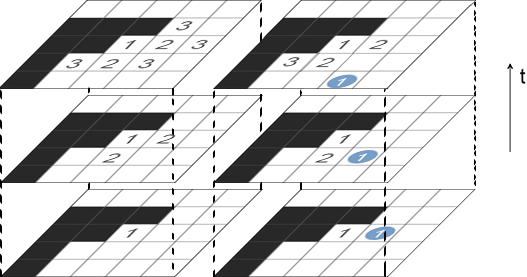
\includegraphics[width=9cm]{images/extended_occupancy.png}
    \centering
    \caption{Beispiele für eine Erreichbarkeitskarte}
    \label{fig:extended_occupancy}
\end{figure}
Abbildung \ref{fig:extended_occupancy} zeigt zwei Erreichbarkeitskarten. Für die linke Karte sind keine Agenten eingetragen. In der rechten Karte ist der geplante Weg für Agent "'1"' eingetragen (in der Abbildung blau). Im Vergleich zeigt sich, dass wegen des Sicherheitsabstand nach zwei Zeitschritten auf der rechten Karte weniger Zellen erreicht werden können.
%
\subsubsection{Der Raum-Zeit-Pfad}
\label{chap:raum-zeit-pfad}
Der Raum-Zeit-Pfad ist das Datenmodell, das die geplanten Wege der Agenten beschreibt \cite{book:regele}. Dieses fußt zwar auf das Weltmodell, stellt sich aber nicht als Gitter dar. Die Positionen werden in einem assoziativen Datenfeld, mit dem Schlüssel \(t\), gespeichert. Zusätzlich zu der Definition des Raum-Zeit-Pfades wird in diesem Kapitel kurz erläutert, wie dieser bestimmt wird.

Zu erst wird die Umgebungskarte um zeitlich um \(t\) verschoben und räumlich so, dass die aktuelle Position des Agenten im Zentrum der Umgebungskarte liegt. Dann werden die alten Raum-Zeit-Pfade der anderen Agenten durch die neuen ersetzt. Jetzt kann die Erreichbarkeitskarte entwickelt werden. Um den eigentlichen Weg zu planen, wird nun die letzte Zeitebene der Erreichbarkeitskarte betrachtet. Von den Zellen, die erreichbar sind, also einen Wert halten, wird die ausgesucht, die den kleinsten Entfernung in der Entfernungskarte hat. Von dieser Zelle aus kann man dann den Weg rückwärts durch die Zeit entwickeln. \cite{book:regele}\newline
Nun kann es aber passieren, dass keine Zelle frei ist, oder dass es zu Konflikten mit anderen Agenten kommt. Das wird im Kapitel \ref{chap:konfliktverarbeitung} vertieft.
\begin{figure}[H]
    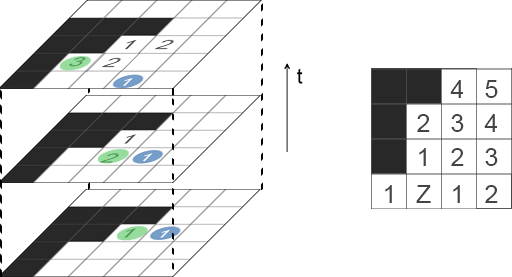
\includegraphics[width=9cm]{images/example_path_planning.png}
    \centering
    \caption{Beispielhafte Wegplanung}
    \label{fig:example_path_planning}
\end{figure}
In Abbildung \ref{fig:example_path_planning} ist die Wegplanung eines Agenten beispielhaft dargestellt. Die Abbildung besteht aus drei Teilen. Zum einen links, die Erreichbarkeitskarte (aus Abbildung \ref{fig:extended_occupancy}), in grün markiert der geplante Weg und rechts ein relevanter Ausschnitt aus der zugehörigen Entfernungskarte (aus Abbildung \ref{fig:distance_localmap}). Die Zelle, die in der Erreichbarkeitskarte in drei Schritten erreichbar ist, besitzt die geringste Entfernung zum globalen Ziel. Diese wird als lokales Ziel markiert. Von hieraus kann nun in der Erreichbarkeitskarte der Weg rückwärts durch die Zeit, hin zur aktuellen Position des Agenten entwickelt werden.

%
\subsection{Konfliktverarbeitung}
\label{chap:konfliktverarbeitung}
Die Agenten des \textit{CoDy Algorithmus} sind kooperativ. Sie sind also in der Lage die eigenen "'Bedürfnisse"' zurückzustellen. Man kann zwischen passiver und aktiver Kooperation unterscheiden. Bei der aktiven Kooperation kann ein Agent die Planung übernehmen und bei anderen Agenten nach Zustimmung oder Ablehnung fragen. Bei der passiven Kooperation müssen alle in einem Konflikt beteiligten Agenten die gesamte Situation berechnen und dann anschließend in einer Verhandlung ihre Lösungen diskutieren. Die passive Kooperation hat gegenüber der aktiven Kooperation vor allem den Vorteil, dass der Kommunikationsaufwand deutlich geringer ist. Sie ist aber auch robuster und der Berechnungsaufwand, so wie sie im CoDy Algorithmus umgesetzt ist, geringer. Die echte passive Kooperation kann sehr ineffizient sein. Deshalb benutzt der CoDy Algorithmus eine abgewandelte Form. Agenten, die potenziell in einen Konflikt geraten können, kommunizieren in einer festen Reihenfolge (siehe Kapitel \ref{chap:kommunikation}) und planen nur ihre eigenen Wege. \cite{book:regele}\newline Folgende Beispielsituation:
Agent "'0"' überschreibt einen Teil des geplanten Weges von Agent "'1"'. Dann schickt Agent "'0"' seinen neuen Plan an alle Agenten. Wenn Agent "'1"' wieder an der Reihe ist, plant dieser mit den neuen Daten. Wann welcher Agent, welche Wege überschreiben kann, wird in Kapitel \ref{chap:prioritaeten} beschrieben.

\subsection{Kommunikation}
\label{chap:kommunikation}
Wie bereits erwähnt, kommunizieren die Agenten in einer festen Reihenfolge. In diesem Kapitel wird beschrieben, wie sich dieser verkette Ablauf ergibt.
Jeder Agent merkt sich mit einem Zeitstempel, wann er mit seinem Berechnungsschritt begonnen hat. Nachdem ein Agent seinen Weg geplant hat, verschickt er den geplanten Weg und den Zeitstempel an alle Agenten und wartet auf Nachrichten der anderen Agenten. Wenn ein Agent eine Nachricht erhält, wird zunächst geprüft, ob sich die Umgebungskarten überschneiden. Wenn dies nicht der Fall ist, wird die Nachricht verworfen, da die Agenten sich nicht beeinflussen. Wenn aber eine Überschneidung festgestellt wird, werden die Zeitstempel mit einander verglichen. Hat der andere Agent früher mit seiner Wegplanung begonnen, muss auf diesen gewartet werden, bevor mit dem Planen der nächsten Wegschritte begonnen wird. Sind beide Zeitstempel gleich, entscheidet die numerische Identifikationsnummer der Agenten. Kleine Nummern sind besser. Somit ergibt sich ein zufälliger, aber fester verketteter Ablauf. Agenten reihen sich also in diesen Ablauf ein, wenn sich die Umgebungskarten überschneiden. Wenn sich die Agenten aber soweit von einander entfernen, dass keine Überschneidung mehr vorliegt, werden sie aus der Kette gelöscht. Durch dieses Vorgehen ist die Entwicklung der Prioritäten, das Hauptwerkzeug der Agenten, um Konflikte zu lösen, vorhersehbar. Dieser Vorteil wiegt mehr, als der Nachteil für diese Bereiche die parallele Berechnung aufzugeben. \cite{book:regele}
%
\subsection{Prioritäten}
\label{chap:prioritaeten}
Agenten sind in der Lage geplante Wege anderer Agenten zu überschreiben. Dies wird durch die Prioritätswerte der Agenten ermöglicht. Wenn die Erreichbarkeitskarte erstellt wird, werden Zellen die von Agenten mit niedrigerer Priorität als die eigene reserviert sind als frei betrachtet. Bei Planen des Wegs wird aber darauf geachtet, dass möglichst wenig Wege überschrieben werden. Wenn zum Beispiel zwei Zellen die Entfernung zum Ziel gleicher maßen verringern und eine von diesen Zellen tatsächlich frei ist, dann wird diese gewählt. \cite{book:regele}

Die dynamische Anpassung der Prioritäten passiert genau dann, wenn ein Konflikt beziehungsweise eine Blockade erkannt wird. Die Konflikterkennung ist dabei recht simpel. Um einen Konflikt zu erkennen, betrachtet man den vom Agenten geplanten Weg. Wenn jeder geplante Schritt den Abstand zum Ziel verringert, liegt \textbf{keine Blockade} vor. Der Prioritätswert wird um den Wert \(PrioNoBlock\) dekrementiert. Der Prioritätswert eines Agenten kann dabei den Wert \(BasePrio\) nicht unterschreiten. Das Dekrementieren des Prioritätswert geschieht, da der Agent eventuell andere Agenten blockiert. Wenn der geplante Weg Schritte enthält, die die Entfernung zum Ziel nicht verbessern, der Agent aber bis zum Schluss in Bewegung bleibt, handelt es sich um einen \textbf{Umweg}. In diesem Fall wird die Priorität nicht verändert, da die Agenten ja kooperativ arbeiten und Umwege in Kauf genommen werden sollen. Wenn der geplante Weg in einer Wartephase endet, handelt es sich um eine \textbf{Blockade}. Da es Agenten aber möglich sein soll, andere Agenten verdrängen zu können, wird eine Blockade nur als solche erkannt, wenn in zwei aufeinander folgenden Berechnungsschritten die gleiche Blockade erkannt wird. In diesem Fall wird die Priorität des Agenten um \(PrioBlock\) erhöht. Mit dieser neuen Priorität plant der Agent erneut seinen Weg. Wichtig ist, dass die Priorität sich nur einmal erhöht. Diese erneute Planung ist für den Berechnungsschritt also die Finale. Wenn kein Weg gefunden wird, also nicht einmal das Verharren auf der eigenen Position möglich ist, dann liegt eine \textbf{total Blockade vor}. In diesem Fall wird die Priorität um \(PrioFullBlock\) erhöht und die Wegplanung erneut durchgeführt. Wenn immer noch kein gültiger Wegeplan berechnet werden konnte, wird ein Notweg erzwungen. Der Notweg ist das Verharren auf der eigenen Position. Zusätzlich wird die Priorität maximal erhöht, damit der Notweg nicht direkt überschrieben werden kann. Für das Überschreiben der Wege ist noch wichtig, dass die ersten drei Zeitschritte geschützt sind. In diesen ersten Zeitschritten dürfen keine Wege anderer Agenten überschrieben werden. Diese Regel gilt jedoch nicht für das Erzwingen eines Notweges. \cite{book:regele}



%
\subsection{Algorithmus}
\label{chap:algorithmus}
In diesem Kapitel werden die zuvor erläuterten Elemente in Kontext gesetzt. 

Wenn die Agenten initialisiert werden, sind ihnen die statischen Hindernisse und die eigene Position bereits bekannt. Alle Agenten werden mit den gleichen Parametern erzeugt. Weil für den ersten Berechnungsschritt die Agenten die Positionen der anderen nicht kennen, planen alle Agenten stehen zu bleiben. Ein Agent führt periodisch die nächste geplante Bewegung aus. Zwischen den Bewegungen finden die Berechnungsschritte statt. Für diese Arbeit findet aus Gründen der Übersicht, nur ein Berechnungsschritt pro Bewegungsschritt statt. Parallel zu den Bewegungs- und Berechnungsschritten, empfängt ein Agent die Nachrichten der anderen Agenten. \cite{book:regele}

Ein Berechnungsschritt läuft folgendermaßen ab:\newline
Damit ein Berechnungsschritt beginnen kann, müssen von allen Agenten, auf die gewartet wird, Nachrichten empfangen werden. Wenn das erfüllt ist, wird die Umgebungskarte zeitlich und räumlich zentriert. Darauffolgend werden die neuen geplanten Wege in die Umgebungskarte eingetragen. Jetzt plant der Agent mit Hilfe einer Erreichbarkeitskarte, den eigenen Weg. Prioritätsanpassungen und eventuelle Neuberechnungen werden gemäß \ref{chap:prioritaeten} durchgeführt. Der geplante Weg wird an alle Agenten per Nachricht übermittelt. \cite{book:regele}